\chapter{Análise dos Problemas de Planejamento de TI em Instituições Públicas Brasileiras}
\label{capitulo:analise_dos_problemas}
Ao buscar os fatores que influenciam nas deficiências dos planejamentos de TI de instituições públicas, esta pesquisa adquire caráter multidisciplinar. Apesar de ser uma atividade vinculada aos ativos de tecnologia, o planejamento é um instrumento essencial da administração e absorve a subjetividade do comportamento dos indivíduos participantes. Neste cenário, o método de pesquisa qualitativa \textit{Grounded Theory} é empregado para analisar o problema e extrair resultados fundamentados na realidade.

\citeonline{glaser:68} apontam alguns pontos fortes da \textit{Grounded Theory}: (i) a fundamentação de dados empíricos  aproxima a pesquisa da realidade; (ii) por se tratar de análise de comportamento, é um método efetivo para o estudo do comportamento humano; (iii) possibilita novas perspectivas, pois toma a realidade como referencial teórico ao invés de buscar fundamentação em teorias já existentes.

Cabe aqui relembrar a questão que este trabalho busca responder: ``apesar da obrigatoriedade e dos conhecidos benefícios, o planejamento de TI não é realizado satisfatoriamente nos órgãos públicos federais. A atividade de planejamento envolve aspectos técnicos e sociais, diante disso, pergunta-se: quais os fatores que dificultam o processo de elaboração do planejamento de TI e qual a relação entre tais fatores?''.

Este capítulo tem como objetivo principal narrar o processo de coleta, análise, descoberta dos resultados e avaliação dos mesmos. Destaca-se a aplicação do método \textit{Grounded Theory} na fase de análise dos dados que, por sua natureza, deve ser capaz de fornecer as evidências para auditorias da pesquisa, arguições e reprodução do caminho percorrido pelo pesquisador até os resultados \cite{corbin:98}.

\section{Coleta dos Dados}
%https://goo.gl/rVPuFK

A amostragem de instituições públicas federais tomada para a aplicação do questionário de coleta de dados, representado no \autoref{apendice:a_quest_coleta}, consiste em Universidades Federais (UFs) e Institutos Federais de Educação, Ciência e Tecnologia (IFs). Na época da aplicação do \textit{survey}, o país contava com um total de 63 UFs e 41 IFs. A presente pesquisa contou com a participação de membros de 37 instituições, representando 35,57\% das instituições federais de ensino superior e técnico.

O público alvo ao qual se destinou o questionário é composto de servidores das instituições da amostragem que participaram de equipes de elaboração do PDTI, comitês de TI ou que atuaram como gestores de setores de TI. O total de respondentes do \textit{survey} soma 53 participantes. Para as análises qualitativas, 4 respostas foram descartadas, pois os respondentes deixaram as questões dissertativas em branco. Os dados foram separados em dois grupos, conforme segue:
\begin{itemize}
\item \textbf{Grupo 1 (instituições sem PDTI):} 9 respostas válidas.
\item \textbf{Grupo 2 (instituições com PDTI):} 40 respostas válidas;
\end{itemize}

Em um total de 53 participantes, o gráfico abaixo apresenta a proporção dos cargos efetivos dos servidores participantes da coleta de dados.

\begin{figure}[h]
\centering % para centralizarmos a figura
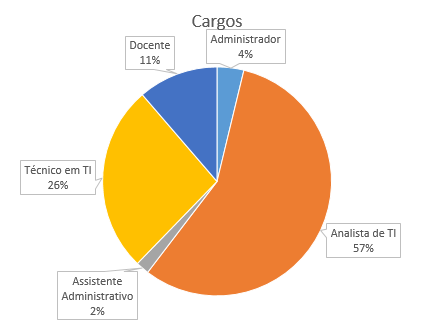
\includegraphics[width=9cm]{figuras/apendiceC_cargos.png}
%\caption{Cargos dos respondentes.}
\end{figure}

Dos 53 participantes, 34 possuem cargo de confiança.

Com relação ao tempo na instituição (em anos), os participantes se distribuem da seguinte forma:
\begin{itemize}
\item 2 anos ou menos: 9 participantes;
\item 3 a 5 anos: 22 participantes;
\item 6 a 10 anos: 14 participantes;
\item 10 a 20 anos: 5 participantes;
\item 20 anos ou mais: 3 participantes.
\end{itemize}

Com relação à formação acadêmica, os participantes estão distribuídos da seguinte forma:
\begin{figure}[h]
\centering % para centralizarmos a figura
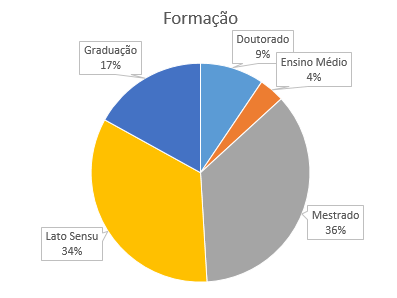
\includegraphics[width=9cm]{figuras/apendiceC_formacao.png}
%\caption{Formação dos respondentes.}
\end{figure}

A Tabela \ref{tabela:resumoColeta} apresenta um resumo da participação no questionário de coleta de dados.

% Please add the following required packages to your document preamble:
% \usepackage{graphicx}
% \usepackage[table,xcdraw]{xcolor}
% If you use beamer only pass "xcolor=table" option, i.e. \documentclass[xcolor=table]{beamer}
\begin{table}[]
\centering
\resizebox{\textwidth}{!}{%
\begin{tabular}{|l|c|c|c|}
\hline
\rowcolor[HTML]{9B9B9B} 
\multicolumn{1}{|c|}{\cellcolor[HTML]{9B9B9B}\textbf{Instituição}} & \textbf{Possui PDTI} & \textbf{Número de respondentes} & \textbf{Respostas válidas} \\ \hline
CEFET-MG                                                           & Sim                  & 1                               & 1                          \\ \hline
IFB                                                                & Sim                  & 1                               & 1                          \\ \hline
IFC                                                                & Sim                  & 7                               & 6                          \\ \hline
IFES                                                               & Sim                  & 1                               & 1                          \\ \hline
IF Farroupilha                                                     & Sim                  & 1                               & 0                          \\ \hline
IFG                                                                & Não                  & 1                               & 1                          \\ \hline
IF Goiano                                                          & Sim                  & 1                               & 1                          \\ \hline
IFMA                                                               & Sim                  & 2                               & 2                          \\ \hline
IFMT                                                               & Sim                  & 3                               & 3                          \\ \hline
IFPE                                                               & Não                  & 2                               & 2                          \\ \hline
IFPI                                                               & Não                  & 2                               & 1                          \\ \hline
IFPR                                                               & Sim                  & 1                               & 1                          \\ \hline
IFRO                                                               & Sim                  & 1                               & 1                          \\ \hline
IFRS                                                               & Sim                  & 1                               & 1                          \\ \hline
IFS                                                                & Sim                  & 1                               & 1                          \\ \hline
IFSC                                                               & Sim                  & 3                               & 3                          \\ \hline
IF Sudeste MG                                                      & Sim                  & 3                               & 3                          \\ \hline
UFAL                                                               & Sim                  & 1                               & 1                          \\ \hline
UFC                                                                & Sim                  & 1                               & 1                          \\ \hline
UFERSA                                                             & Sim                  & 1                               & 1                          \\ \hline
UFFS                                                               & Sim                  & 1                               & 1                          \\ \hline
UFGD                                                               & Sim                  & 1                               & 1                          \\ \hline
UFJF                                                               & Sim                  & 1                               & 0                          \\ \hline
UFOB                                                               & Não                  & 1                               & 1                          \\ \hline
UFPA                                                               & Não                  & 1                               & 1                          \\ \hline
UFPB                                                               & Sim                  & 1                               & 1                          \\ \hline
UFPE                                                               & Sim                  & 1                               & 1                          \\ \hline
UFRGS                                                              & Sim                  & 1                               & 1                          \\ \hline
UFRPE                                                              & Sim                  & 1                               & 1                          \\ \hline
UFRR                                                               & Não                  & 1                               & 1                          \\ \hline
UFS                                                                & Sim                  & 1                               & 1                          \\ \hline
UFSJ                                                               & Não                  & 1                               & 1                          \\ \hline
UFSM                                                               & Sim                  & 2                               & 2                          \\ \hline
UFTM                                                               & Sim                  & 1                               & 1                          \\ \hline
UFTO                                                               & Sim                  & 1                               & 1                          \\ \hline
UNIFESSPA                                                          & Não                  & 1                               & 1                          \\ \hline
UTFPR                                                              & Sim                  & 1                               & 1                          \\ \hline
\end{tabular}%
}
\caption{Instituições participantes da pesquisa.}
\label{tabela:resumoColeta}
\end{table}

O questionário foi elaborado levando em consideração a existência de instituições que possuem o PDTI, enquanto outras não possuem. A plataforma eletrônica escolhida para a aplicação do \textit{survey} permitiu o direcionamento do respondente para as questões de acordo com a situação do PDTI de sua instituição. O processo de elaboração do PDTI descrito no ``Guia do PDTI'' do SISP, orientou a ordem e o conteúdo das questões.

O grupo 1 possui apenas uma questão dissertativa: ``Quais os impedimentos ou dificuldades que a gestão de TI da sua instituição encontrou que justifique a falta de um PDTI?''. Os respondentes produziram o material de análise do grupo 1 ao responder a este questionamento.

O grupo 2 possui cinco questões dissertativas, como segue abaixo:
\begin{itemize}
\item A respeito do diagnóstico das necessidades de TI da instituição, fale sobre as dificuldades encontradas durante o processo de levantamento de necessidades na sua instituição;
\item Fale sobre as dificuldades encontradas na elaboração de critérios e priorização das necessidades da sua instituição;
\item Fale sobre as dificuldades encontradas na etapa de definição de metas e ações;
\item Fale sobre as dificuldades encontradas na etapa de planejar o gerenciamento de riscos;
\item Comente sobre qualquer outra dificuldade que tenha chegado ao seu conhecimento que a equipe que participou da elaboração ou revisão do PDTI tenha enfrentado.
\end{itemize}

O questionário é composto de questões objetivas e dissertativas sobre a elaboração do Plano Diretor de TI nas respectivas instituições dos respondentes. As questões objetivas tem o intuito de informar dados sobre os participantes, além de fornecer parâmetros quantitativos sobre o tema pesquisado, como pode ser visualizado no relatório do \autoref{apendice:c_relat_quantitativo}. As questões dissertativas, foco desta pesquisa, tem o objetivo de coletar os relatos dos participantes sobre suas experiências com o PDTI. Estas respostas, presentes no \autoref{apendice:d_respostas_disserta}, são os dados de entrada para a etapa de análise descrita na seção seguinte.

\section{Análise: Aplicação do Método Grounded Theory}

\begin{citacao}
Embora não criemos dados, criamos teoria a partir dos dados. Se fizermos isso corretamente, então não estaremos falando para nossos participantes, mas, sim, permitindo que eles falem com vozes claramente entendidas e representativas. Nossas teorias, embora imcompletas, fornecem uma linguagem comum (conjunto de conceitos) por meio da qual participantes da pesquisa, profissionais e outros podem se reunir para discutir ideias e encontrar soluções para os problemas \cite{corbin:98}.
\end{citacao}

Para analisar os dados, principalmente nas fases iniciais do método, utilizou-se da técnica de microanálise\footnote{Análise detalhada dos dados coletados, linha por linha ou palavra por palavra, necessária no começo de um estudo para gerar as primeiras categorias \cite{corbin:98}.}. Esta técnica consiste em buscar significado em pequenas porções dos dados, frases ou até mesmo palavras, de forma isolada do restante do texto. \citeonline{corbin:98} sugere que o pesquisador pergunte: ``O que esta palavra parece significar, ou o que ela poderia significar?''. Este exercício permite que o pesquisador busque por significados fora dos modos usuais, tornando-o consciente do quanto está contido em pequenas quantias de dados.

A microanálise evita que se tome partido ou que se assuma uma posição em relação aos dados. O pesquisador, desta forma, é forçado a pensar fora do senso comum e, com isso, o dado se mantém isolado sem ser forçado a assumir um conceito baseado em contexto. As falsas suposições ou significados atribuídos inicialmente sobre os dados não se sustentam, pois os dados são confrontados e comparados uns com os outros na medida em que se avança a análise \cite{corbin:98}.

As subseções seguintes tem o objetivo de narrar a análise dos dados coletados utilizando as fases da \textit{Grounded Theory} como arcabouço. Esta etapa da pesquisa, objetivando ser fiel ao método GT, buscou referências em livros textos e trabalhos acadêmicos acerca do método. As referências utilizadas para a aplicação do método de análise foram \citeonline{strauss:87}, \citeonline{corbin:98}, \citeonline{bandeira:03}, \citeonline{conte:09} e \citeonline{schots:10}.

	\subsection{Codificação aberta}
	
\citeonline{corbin:98} definem a codificação aberta como um processo analítico através do qual conceitos são identificados nos dados e suas propriedades e dimensões são descobertas. Nesta etapa trabalha-se com a ideia de 
códigos. ``Um código representa um conceito que dá significado a um trecho do documento, podendo se referir a uma citação, objeto, evento, problema, aspecto ou situação'' \cite{schots:10}.

O primeiro passo tomado na codificação aberta é a leitura completa do material coletado, que no caso desta pesquisa trata-se de um conjunto de respostas no formato texto, conforme apresentado no \autoref{apendice:d_respostas_disserta}. A leitura inicial permite uma visão geral do material de análise.

Os autores de \textit{Grounded Theory} indicam eleger um documento base após a leitura inicial, ou seja, um documento mais completo, mais rico em conceitos \cite{strauss:87,corbin:98}. O objetivo desta atividade é estabelecer os primeiros códigos que, posteriormente, ganharão densidade ao serem observados nos demais documentos. No caso desta pesquisa, há apenas um documento para cada grupo de análise. Diante disso, optou-se por começar a codificação pelas respostas mais completas, mais ricas em conceitos em cada um dos grupos. No grupo 1, a análise iniciou pela resposta cujo identificador é ID-3. Já no grupo 2, foi eleita a resposta de identificador ID-9 da primeira questão. Ambas respostas são transcritas a seguir.

\textit{\textbf{Grupo 1, resposta ID-3:} ``Falta de iniciativa e incentivo da alta gestão; Falta de plano estratégico institucional objetivo; Falta de pessoal voltado especificamente a área de planejamento e governança''.}

\textit{\textbf{Grupo 2, questão 1, resposta ID-9:} ``O inventário de necessidades é realizado por equipes nos Campi e Reitoria. No geral, encontram-se dificuldades em se estabelecer reuniões objetivas com os clientes do negócio. Muitas vezes os mesmos superestimam as necessidades dado algum receio de que não haja ``outra oportunidade''  para comprar bens e serviços em TI. Também é difícil ter que fazer compreender que as necessidades devem estar alinhadas aos objetivos estratégico e não desejos dos usuários''.}

Ao aplicar a técnica de microanálise nos dados citados acima, originaram-se os primeiros códigos. A resposta ID-3, por exemplo, originou os seguintes códigos: ``Falta PEI'', ``Alta gestão imatura'', ``Falta de iniciativa'', ``Falta de incentivo'' e ``Falta equipe especialista''.

Para cada código gerado, foi redigido um comentário descrevendo as características do conceito que representa tal código. Além disso, o comentário contém os critérios que permitam a uma citação ser candidata a se ligar a este código. Por exemplo, o comentário do código ``Alta gestão imatura''  apresenta o seguinte conteúdo:

\textit{\textbf{Código - Alta gestão imatura:}
Conceito que se refere a imaturidade estratégica da cúpula administrativa de uma instituição. Setor ligado à alta administração, tomadores de decisões estratégicas da instituição.
Este código pode ser aplicado em situações onde os dados façam referência à deficiência estratégica por parte da reitoria e/ou pró-reitorias. Os setores de TI não estão inclusos neste conjunto.}

Os comentários de todos os códigos desta pesquisa são apresentados no \autoref{apendice:e_codigos}.

Durante o processo de microanálise na busca por códigos, são feitos questionamentos aos dados e comparações teóricas com situações semelhantes para que haja uma minuciosa examinação e interpretação dos dados. Isto permite melhor compreensão do conceito e faz com que as propriedades e dimensões dos códigos emerjam dos dados \cite{corbin:98}. Tais questionamentos e comparações feitas foram registradas em notas (\textit{memos}), que nesta fase, são chamadas de notas de microanálise (MA). Também deve constar nos \textit{memos} MA, toda a descrição do processo de validação dos questionamentos e proposições buscando citações no formulário analisado ou nos demais, trata-se da fundamentação nos dados. Abaixo, um exemplo de uma nota do tipo MA:

\textit{\textbf{MA Códigos ``Falta de iniciativa''  e ``Falta de incentivo'': }}
\textit{
estes códigos parecem significar que falta de iniciativa e/ou de incentivo são causas para a falta de um PDTI. Quem deveria tomar esta iniciativa? Este tipo de resposta seria uma transferência de culpa? Deixa a sensação de que se houvesse o ``primeiro passo'', o PDTI teria acontecido. A alta gestão não incentiva a criação do PDTI, será que esta instituição não recebeu recomendações do TCU ou orientações do SISP que fomentam o ``incentivo'' à criação do PDTI?
Fundamentação: a citação do respondente ID3 indica que quem deveria tomar a iniciativa e incentivar seria a alta gestão da instituição, ou seja, a iniciativa não é da própria equipe de TI e o incentivo deve partir da alta gestão. 
O respondente do ID23, cita que há cobranças de órgãos de controle, isto é um ``incentivo'' a se criar o PDTI.}

Todas as notas de microanálise desta pesquisa são apresentadas no \autoref{apendice:f_notas_ma}.

O documento base serviu para registrar os primeiros códigos. O processo de codificação, incluindo as anotações de comentários e microanálise, foi aplicado nas demais respostas fazendo comparações com aquelas já analisadas e com os novos códigos registrados de forma recursiva. O processo de codificação, apesar de ser descrito de forma sequencial neste trabalho, ocorre de forma iterativa, conforme ilustra a Figura \ref{figura:gt_iterativo}.

\begin{figure}[h]
\centering % para centralizarmos a figura
\includegraphics[width=15cm]{figuras/gt_iterativo.png}
\caption{Processo de análise, extraído de \citeonline{bandeira:03}.}
\label{figura:gt_iterativo}
\end{figure}

Nesta etapa da codificação aberta a pesquisa apresenta: (i) a validação de códigos criados anteriormente; (ii) incremento do número de citações relacionadas a um determinado código; (iii) a criação de novos códigos. Uma vez que os códigos vão se acumulando, inicia-se o processo de agrupamento dos códigos ou categorização dos mesmos sob termos mais abstratos, isto é, categorias. A categoria representa um fenômeno observado a partir dos dados e responde a perguntas do tipo ``O que está acontecendo?'' \cite{corbin:98}.

Para encontrar as categorias, os códigos e anotações criados anteriormente foram revistos, analisando aqueles que possuem propriedades em comum que permitam elevar o nível de abstração do fenômeno ali representado, originando categorias. Em um exemplo hipotético apresentado por \citeonline{corbin:98}, os códigos “pássaro”, “pipa” e “avião” possuem uma propriedade em comum, que é a habilidade de voar e, desta forma, podem ser agrupados na categoria “voa”.

As categorias precisam ser descritas em função de suas propriedades e dimensões para facilitar o retorno aos dados, ou seja, servem como critérios para procurar outros códigos que se relacionam com aquela categoria. Propriedade é um atributo da categoria que, em conjunto com outras propriedades, dão significado à categoria. Já a dimensão se trata de uma métrica ou conjunto de valores que uma determinada propriedade da categoria pode assumir \cite{strauss:87}.

Um exemplo de categoria mapeada no grupo 1 é a categoria ``Deficiências na gestão da instituição''. Esta categoria possui a propriedade ``nível de maturidade em gestão na instituição'' que, por sua vez, possui duas dimensões: alta e baixa, onde a primeira indica instituição com indicadores positivos de maturidade na gestão e a segunda, com indicadores negativos de maturidade na gestão. Todos os códigos que tem esta propriedade são candidatos a fazerem parte da categoria.

No grupo 2, um exemplo de categoria mapeada é a categoria ``Problemas com recursos humanos'', cuja propriedade é o ``grau de adequação dos recursos humanos para as atividades de planejamento de TI''. As dimensões para a propriedade desta categoria são: adequado (recursos humanos adequados para as atividades do PDTI) e inadequado (recursos humanos inadequados para as atividades do PDTI).

O conjunto completo das categorias levantadas nesta pesquisa é apresentado no \autoref{apendice:e_codigos}. Após a criação das categorias, retorna-se ao material, explorando-as e fazendo novos questionamentos em busca de detalhar as categorias em subcategorias. Ao final da codificação aberta, é possível observar o mapa de códigos e categorias criados nesta primeira fase de codificação. Tais códigos e categorias estão sujeitos a sofrerem alterações nas fases seguintes da análise. As Figuras \ref{figura:oc_grupo1} e \ref{figura:oc_grupo2} representam o esquema teórico de códigos no momento da conclusão da codificação aberta dos grupos 1 e 2, respectivamente.

\begin{figure}[h]
\centering % para centralizarmos a figura
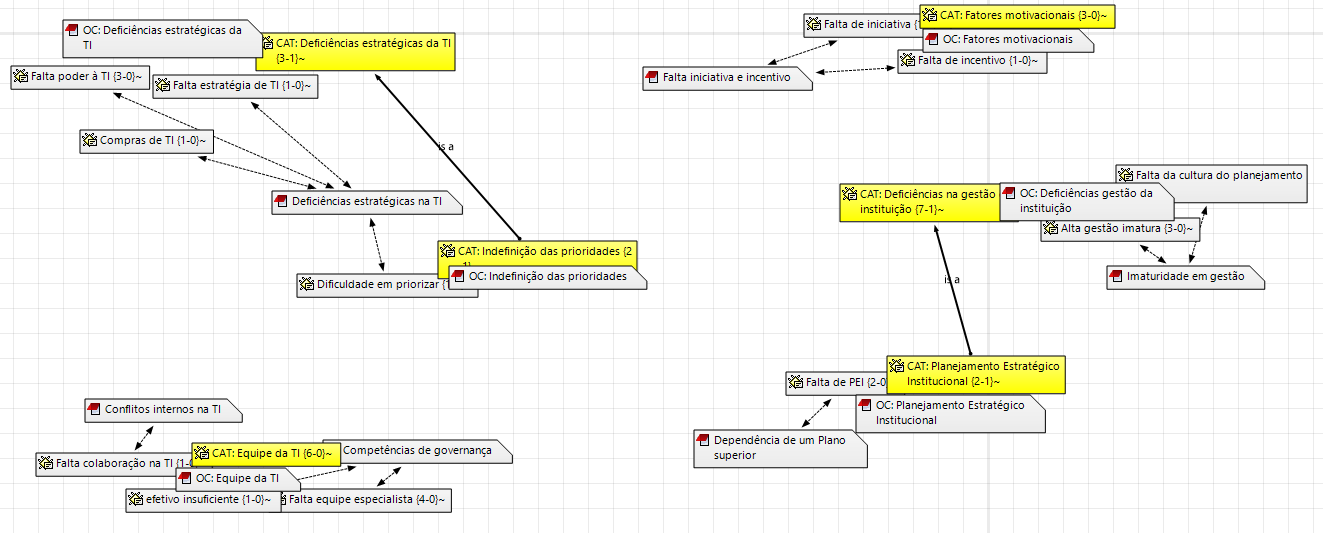
\includegraphics[width=16cm, frame]{figuras/oc_grupo1.PNG}
\caption{Esquema teórico do grupo 1 após a codificação aberta.}
\label{figura:oc_grupo1}
\end{figure}

\begin{figure}[h]
\centering % para centralizarmos a figura
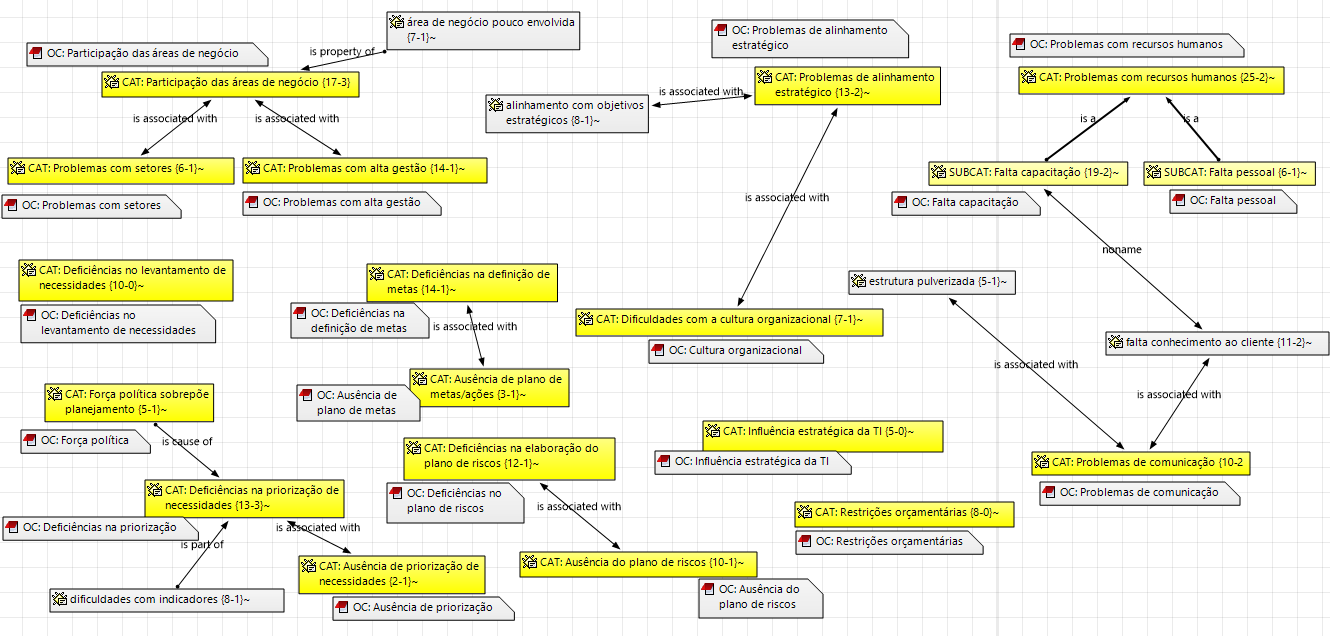
\includegraphics[width=16cm, frame]{figuras/oc_grupo2.PNG}
\caption{Esquema teórico do grupo 2 após a codificação aberta.}
\label{figura:oc_grupo2}
\end{figure}
	
Foram criadas notas de codificação aberta (OC), para cada categoria, contendo as citações que se encaixam em cada dimensão de cada propriedade. As notas do tipo OC também podem conter a narração do processo de retorno aos dados descrevendo os \textit{insights} e quaisquer questionamentos ou interpretações julgadas importantes para registrar o caminho de pensamento que levou a enquadrar determinada citação em determinada propriedade. A Figura \ref{figura:oc_memo} apresenta um trecho de uma das notas do tipo OC da presente pesquisa. 

\begin{figure}[h]
\centering % para centralizarmos a figura
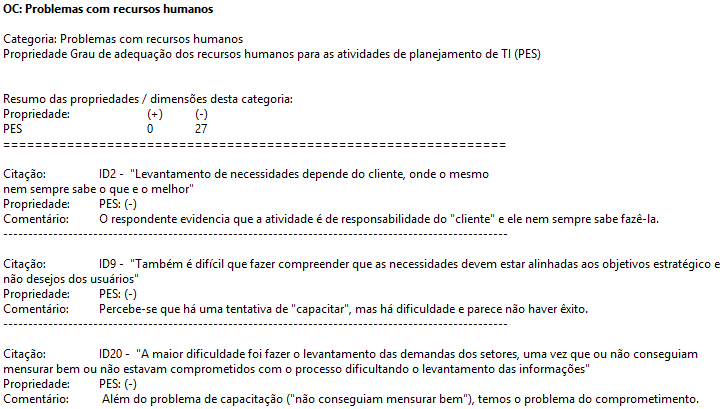
\includegraphics[width=16cm, frame]{figuras/oc_memo.PNG}
\caption{Exemplo de nota de codificação aberta.}
\label{figura:oc_memo}
\end{figure}

Pode-se observar, inclusive que a nota de codificação aberta possui a quantidade de ocorrências de cada dimensão de cada propriedade. Todas as notas do tipo OC podem ser observadas no \autoref{apendice:h_notas_oc}.

Ao final da codificação aberta as categorias estão com propriedades bem definidas e padrões de ocorrência efetivamente encontrados nos dados. Propriedades que não encontraram fundamentação empírica são descartadas e, com isto, categorias também podem ser alteradas ou excluídas. Isto garante a fundamentação empírica.

	\subsection{Codificação axial}
A codificação axial pode ser resumida no processo de relacionar categorias entre si e entre subcategorias. O termo “axial” é usado pois, uma a uma, a categoria é posta em um eixo de análise onde o objetivo é relacioná-la ao nível de propriedades e dimensões \cite{corbin:98}.

De acordo com \citeonline{corbin:98}, começando com análises das primeiras respostas, o pesquisador não deve ajudar, mas observar (e fazer anotações) como os códigos se relacionam. Ao explicar os relacionamentos, cria-se ligações entre categorias e suas subcategorias. Este procedimento permite verificar se os relacionamentos parecem ser condições, ações/interações ou consequências. Estes três elementos formam o que os autores chamam de paradigma \cite{conte:09}. Aos palpites iniciais formados por paradigmas, dá-se o nome de hipóteses ou proposições, pois eles ligam dois ou mais conceitos, explicando o que, porquê, onde, e como do fenômeno.

Na prática, esta etapa consiste em analisar uma categoria por vez, buscando relacionar com suas subcategorias identificando os códigos que representam condições, ações/interações e consequências. Para isso, é interessante ``quebrar'' a categoria em questão expondo seus códigos (propriedades, dimensões e subcategorias). As ligações entre cada código foram rotuladas, seguindo uma convenção de conectores, conforme apresentado na \autoref{secao:principios_da_gt}.

Após mapear os relacionamentos categorias-subcategorias de todas as categorias, o mesmo processo foi aplicado para mapear os relacionamentos entre categorias. Sempre que identificado um relacionamento, os \textit{insights}, os questionamentos e a lógica de pensamento que estruturou o relacionamento foram relatados em anotações, nesta etapa, chamadas de notas de codificação axial (AC). 

Há uma nota do tipo AC para cada relacionamento e nela contém proposições, ou hipóteses que passam por validação nos dados. As hipóteses foram estruturadas usando os elementos: condições, ações/interações e consequências. Após a criação de todos relacionamentos, com suas respectivas notas do tipo AC, retornou-se aos dados para buscar nos formulários de respostas evidências que dão veracidade à cada hipótese descrita nas anotações. Todas as notas AC desta pesquisa são apresentadas no \autoref{apendice:i_notas_ac}. A Figura \ref{figura:ac_memo} ilustra uma destas anotações.

\begin{figure}[h!]
\centering % para centralizarmos a figura
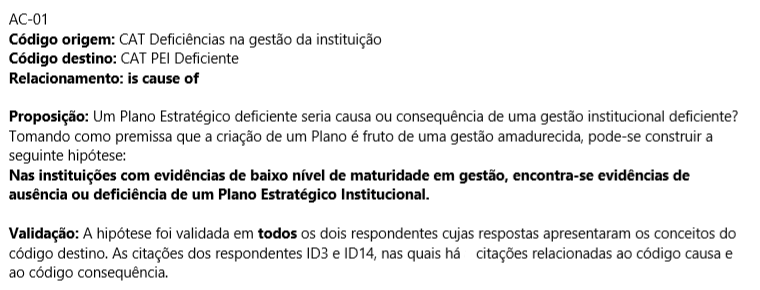
\includegraphics[width=16cm, frame]{figuras/ac_memo.PNG}
\caption{Exemplo de nota de codificação axial.}
\label{figura:ac_memo}
\end{figure}

As Figuras \ref{figura:ac_grupo1} e \ref{figura:ac_grupo2} representam o esquema teórico com as categorias e seus relacionamentos, no momento da conclusão da codificação axial dos grupos 1 e 2, respectivamente.

\begin{figure}[!ht]
\centering % para centralizarmos a figura
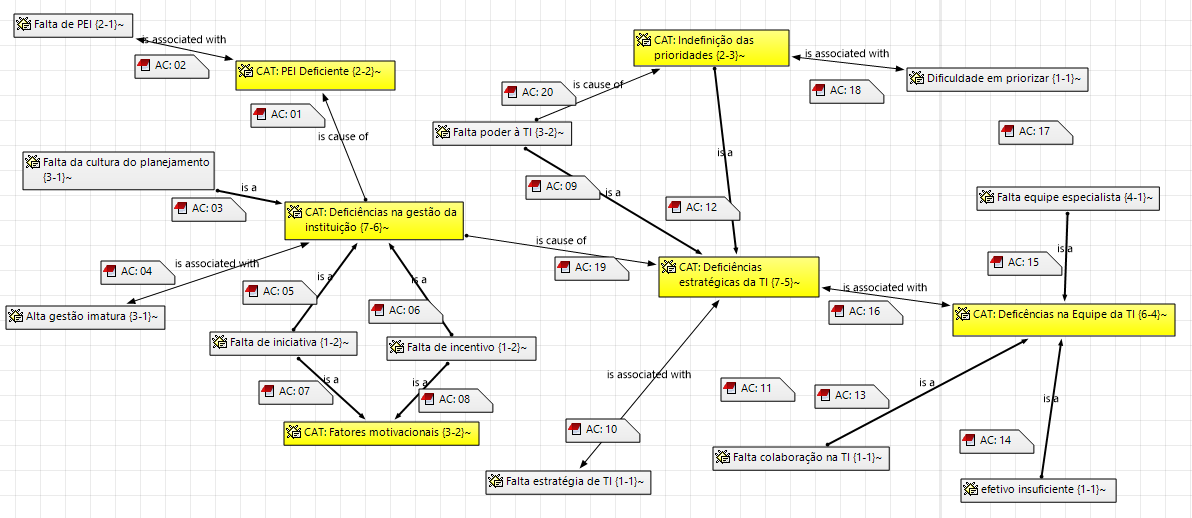
\includegraphics[width=16cm, frame]{figuras/ac_grupo1.PNG}
\caption{Esquema teórico do grupo 1 após a codificação axial.}
\label{figura:ac_grupo1}
\end{figure}

\begin{figure}[!ht]
\centering % para centralizarmos a figura
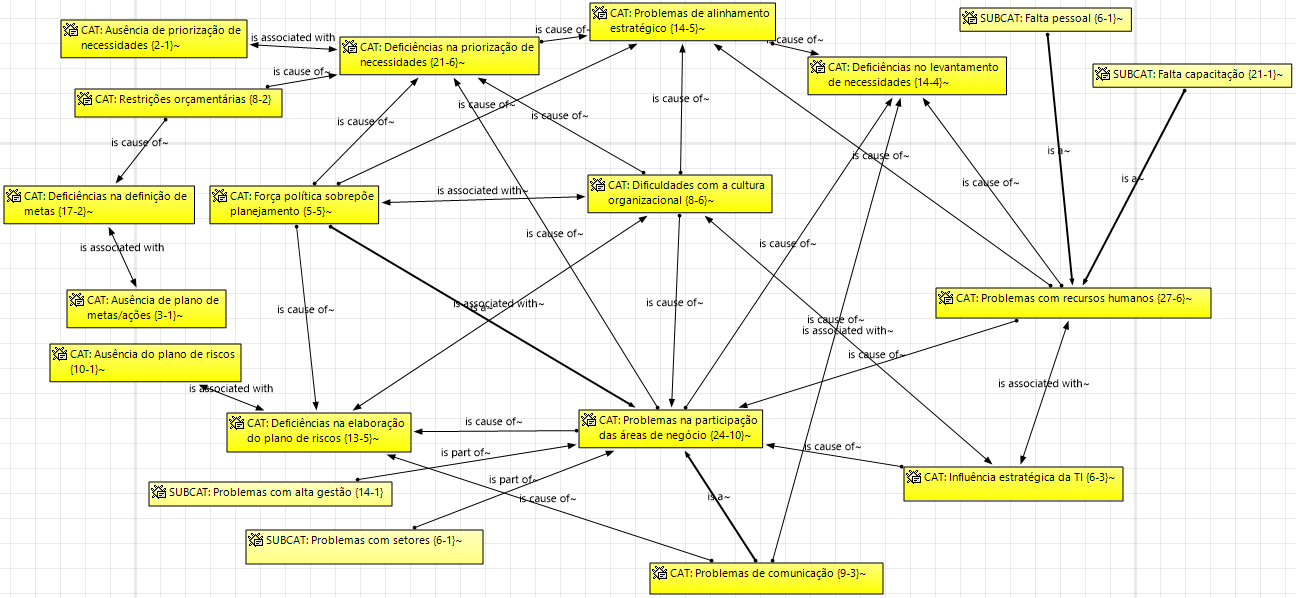
\includegraphics[width=16cm, frame]{figuras/ac_grupo2.PNG}
\caption{Esquema teórico do grupo 2 após a codificação axial.}
\label{figura:ac_grupo2}
\end{figure}

As Tabelas \ref{tabela:relacionamentos_teoria1} e \ref{tabela:relacionamentos_teoria2} apresentam os relacionamentos entre as categorias ao final da etapa de codificação axial.

\begin{table}[H]
\centering
\resizebox{\textwidth}{!}{%
\begin{tabular}{|
>{\columncolor[HTML]{C0C0C0}}l |l|l|l|l|}
\hline
\multicolumn{1}{|c|}{\cellcolor[HTML]{C0C0C0}\textbf{Categoria}}                 & \multicolumn{1}{c|}{\cellcolor[HTML]{C0C0C0}\textbf{is a}}                 & \multicolumn{1}{c|}{\cellcolor[HTML]{C0C0C0}\textbf{is cause of}}                               & \multicolumn{1}{c|}{\cellcolor[HTML]{C0C0C0}\textbf{is associated with}}   & \multicolumn{1}{c|}{\cellcolor[HTML]{C0C0C0}\textbf{is part of}} \\ \hline
PEI Deficiente                                                                   &                                                                            &                                                                                                 &                                                                            &                                                                  \\ \hline
\begin{tabular}[c]{@{}l@{}}Deficiências na \\ gestão da instituição\end{tabular} &                                                                            & \begin{tabular}[c]{@{}l@{}}PEI Deficiente;\\ \\ Deficiências \\ estratégicas da TI\end{tabular} &                                                                            &                                                                  \\ \hline
Fatores motivacionais                                                            &                                                                            &                                                                                                 &                                                                            &                                                                  \\ \hline
\begin{tabular}[c]{@{}l@{}}Indefinição das \\ prioridades\end{tabular}           & \begin{tabular}[c]{@{}l@{}}Deficiências \\ estratégicas da TI\end{tabular} &                                                                                                 &                                                                            &                                                                  \\ \hline
\begin{tabular}[c]{@{}l@{}}Deficiências \\ estratégicas da TI\end{tabular}       &                                                                            &                                                                                                 & \begin{tabular}[c]{@{}l@{}}Deficiências \\ na equipe da TI\end{tabular}    &                                                                  \\ \hline
\begin{tabular}[c]{@{}l@{}}Deficiências\\ na equipe da TI\end{tabular}           &                                                                            &                                                                                                 & \begin{tabular}[c]{@{}l@{}}Deficiências \\ estratégicas da TI\end{tabular} &                                                                  \\ \hline
\end{tabular}%
}
\caption{Relacionamentos entre categorias ao final da codificação axial da teoria 1.}
\label{tabela:relacionamentos_teoria1}
\end{table}

% Please add the following required packages to your document preamble:
% \usepackage{graphicx}
% \usepackage[table,xcdraw]{xcolor}
% If you use beamer only pass "xcolor=table" option, i.e. \documentclass[xcolor=table]{beamer}
\begin{table}[H]
\centering
\resizebox{\textwidth}{!}{%
\begin{tabular}{|
>{\columncolor[HTML]{C0C0C0}}l |l|l|l|l|}
\hline
\multicolumn{1}{|c|}{\cellcolor[HTML]{C0C0C0}\textbf{Categoria}}                          & \multicolumn{1}{c|}{\cellcolor[HTML]{C0C0C0}\textbf{is a}}                               & \multicolumn{1}{c|}{\cellcolor[HTML]{C0C0C0}\textbf{is cause of}}                                                                                                                                & \multicolumn{1}{c|}{\cellcolor[HTML]{C0C0C0}\textbf{is associated with}}                                                               & \multicolumn{1}{c|}{\cellcolor[HTML]{C0C0C0}\textbf{is part of}} \\ \hline
\begin{tabular}[c]{@{}l@{}}Ausência de priorização\\  de necessidades\end{tabular}        &                                                                                          &                                                                                                                                                                                                  & \begin{tabular}[c]{@{}l@{}}Deficiências na priorização\\ de necessidades\end{tabular}                                                  &                                                                  \\ \hline
Restrições orçamentárias                                                                  &                                                                                          & \begin{tabular}[c]{@{}l@{}}Deficiências na priorização\\ de necessidades;\\ \\ Deficiências na definição\\ de metas\end{tabular}                                                                 &                                                                                                                                        &                                                                  \\ \hline
\begin{tabular}[c]{@{}l@{}}Deficiências na definição\\ de metas\end{tabular}              &                                                                                          &                                                                                                                                                                                                  & \begin{tabular}[c]{@{}l@{}}Ausência de plano de\\ metas/ações\end{tabular}                                                             &                                                                  \\ \hline
\begin{tabular}[c]{@{}l@{}}Ausência de plano de\\ metas/ações\end{tabular}                &                                                                                          &                                                                                                                                                                                                  & \begin{tabular}[c]{@{}l@{}}Deficiências na definição\\ de metas\end{tabular}                                                           &                                                                  \\ \hline
\begin{tabular}[c]{@{}l@{}}Ausência do plano de\\ riscos\end{tabular}                     &                                                                                          &                                                                                                                                                                                                  & \begin{tabular}[c]{@{}l@{}}Deficiências\\ na elaboração do plano\\ de riscos\end{tabular}                                              &                                                                  \\ \hline
\begin{tabular}[c]{@{}l@{}}Deficiências\\ na elaboração do plano\\ de riscos\end{tabular} &                                                                                          &                                                                                                                                                                                                  & \begin{tabular}[c]{@{}l@{}}Ausência do plano de\\ riscos;\\ \\ Dificuldades com a cultura\\ organizacional\end{tabular}                &                                                                  \\ \hline
\begin{tabular}[c]{@{}l@{}}Força política sobrepõe\\ planejamento\end{tabular}            & \begin{tabular}[c]{@{}l@{}}Problemas na participação\\ das áreas de negócio\end{tabular} & \begin{tabular}[c]{@{}l@{}}Deficiências na priorização\\ de necessidades;\\ \\ Problemas de alinhamento\\ estratégico;\\ \\ Deficiências na elaboração\\ do plano de riscos\end{tabular}         & \begin{tabular}[c]{@{}l@{}}Dificuldades com a cultura\\ organizacional\end{tabular}                                                    &                                                                  \\ \hline
\begin{tabular}[c]{@{}l@{}}Deficiências na priorização\\ de necessidades\end{tabular}     &                                                                                          & \begin{tabular}[c]{@{}l@{}}Problemas de alinhamento\\ estratégico;\end{tabular}                                                                                                                  & \begin{tabular}[c]{@{}l@{}}Ausência de priorização\\  de necessidades\end{tabular}                                                     &                                                                  \\ \hline
\begin{tabular}[c]{@{}l@{}}Problemas de alinhamento\\ estratégico\end{tabular}            &                                                                                          &                                                                                                                                                                                                  &                                                                                                                                        &                                                                  \\ \hline
\begin{tabular}[c]{@{}l@{}}Dificuldades com a cultura\\ organizacional\end{tabular}       &                                                                                          & \begin{tabular}[c]{@{}l@{}}Deficiências na priorização\\ de necessidades;\\ \\ Problemas de alinhamento\\ estratégico;\\ \\ Problemas na participação\\ das áreas de negócio\end{tabular}        & \begin{tabular}[c]{@{}l@{}}Deficiências\\ na elaboração do plano\\ de riscos;\\ \\ Força política sobrepõe\\ planejamento\end{tabular} &                                                                  \\ \hline
\begin{tabular}[c]{@{}l@{}}Problemas na participação\\ das áreas de negócio\end{tabular}  &                                                                                          & \begin{tabular}[c]{@{}l@{}}Deficiências no levantamento\\ de necessidades;\\ \\ Deficiências na priorização\\ de necessidades;\\ \\ Deficiências na elaboração\\ do plano de riscos\end{tabular} &                                                                                                                                        &                                                                  \\ \hline
Problemas de comunicação                                                                  & \begin{tabular}[c]{@{}l@{}}Problemas na participação\\ das áreas de negócio\end{tabular} & \begin{tabular}[c]{@{}l@{}}Deficiências na elaboração\\ do plano de riscos;\\ \\ Deficiências no levantamento\\ de necessidades\end{tabular}                                                     &                                                                                                                                        &                                                                  \\ \hline
\begin{tabular}[c]{@{}l@{}}Deficiências no levantamento\\ de necessidades\end{tabular}    &                                                                                          &                                                                                                                                                                                                  &                                                                                                                                        &                                                                  \\ \hline
\begin{tabular}[c]{@{}l@{}}Problemas com recursos\\ humanos\end{tabular}                  &                                                                                          & \begin{tabular}[c]{@{}l@{}}Problemas no levantamento\\ de necessidades;\\ \\ Problemas de alinhamento\\ estratégico;\\ \\ Problemas na participação\\ das áreas de negócio\end{tabular}          & \begin{tabular}[c]{@{}l@{}}Influência \\ estratégica da TI\end{tabular}                                                                &                                                                  \\ \hline
Influência estratégica da TI                                                              &                                                                                          & \begin{tabular}[c]{@{}l@{}}Problemas na participação\\ as áreas de negócio\end{tabular}                                                                                                          & \begin{tabular}[c]{@{}l@{}}Problemas com recursos\\ humanos;\\ \\ Dificuldades com a cultura\\ organizacional\end{tabular}             &                                                                  \\ \hline
\end{tabular}%
}
\caption{Relacionamentos entre categorias ao final da codificação axial da teoria 2.}
\label{tabela:relacionamentos_teoria2}
\end{table}

O \textit{software} ``Atlas.ti'', utilizado nesta pesquisa, possui uma ferramenta de consulta (\textit{query}) que se mostrou bastante útil na codificação axial. Com esta ferramenta foi possível mapear os códigos que possuem categorias em comum e, desta forma, que evidenciam o relacionamento entre as categorias. Isto possibilitou manter a fundamentação empírica na codificação axial. 

Ao contar com categorias identificadas e relacionadas entre si, o conhecimento sobre o fenômeno já permite fazer \textit{insights} sobre de que tratam os dados. Essa tarefa é o foco na codificação seletiva, descrita adiante \cite{bandeira:03}.

	\subsection{Codificação seletiva}

\citeonline{corbin:98} definem a codificação seletiva como o processo de integração e refinamento de categorias. É comum, após codificar grande parte dos dados, e identificar as relações entre as categorias, que o pesquisador tenha condições de inferir sobre qual é a categoria central que consegue integrar todas as outras categorias \cite{bandeira:03}.

O primeiro passo para integrar as categorias é decidir (identificar) uma categoria central, que representa o principal tema da pesquisa. De acordo com \citeonline{corbin:98}, a categoria central pode evoluir fora das categorias existentes, ou seja, embora cada categoria da pesquisa seja parte da explicação da teoria, o pesquisador pode concluir que as categorias mapeadas não são suficientes para completar a explicação do fenômeno. Porém, este não foi o caso desta pesquisa, na qual a categoria central é oriunda das fases de codificação anteriores.

Para encontrar a categoria central foram utilizados como referência os seis critérios de \citeonline{strauss:87}. Estes critérios podem ser aplicados a uma categoria para auxiliar na decisão que a qualifica como candidata à categoria central:

\begin{enumerate}
\item Todas as outras categorias principais devem relacionar com ela (a categoria sendo analisada);
\item Ela deve aparecer com frequência nos dados, ou seja, na maioria ou em todos os casos devem existir indicadores apontando para aquele conceito;
\item A explicação que evolui a partir dela relacionando outras categorias deve ser lógica e consistente, sem forçar dados;
\item O nome ou frase usado para descrever a categoria central deve ser suficientemente abstrato ao ponto de permitir ser usado para fazer pesquisa em outras áreas, levando a um desenvolvimento de uma teoria mais geral;
\item Como o conceito é refinado analiticamente através da integração com outros conceitos, a teoria cresce em profundidade e em poder explicativo;
\item O conceito é capaz de explicar variações, assim como o ponto principal, oriundos dos dados. Isto é, quando condições variam, a explicação se mantém, embora a forma com que o fenômeno seja expressado possa observar algo diferente.
\end{enumerate}

Seguindo as orientações de \citeonline{corbin:98}, além das técnicas para se obter a categoria central, é necessário manter uma certa distância dos dados nesta etapa da pesquisa, ou seja, o pesquisador deve desapegar dos detalhes, para que possa se concentrar em extrair uma ideia central, abstrata; também evitou-se reler as anotações pois, segundo os autores, pode confundir o pesquisador com o excesso de informações.

Existem várias técnicas que podem ser usadas para facilitar a identificação da categoria central e a integração de conceitos, dentre elas estão a escrita de enredo (\textit{Storyline}) e o uso de diagramas \cite{corbin:98}. Estas duas técnicas foram aplicadas nesta pesquisa.

O uso de diagramas foi feito desde o início da codificação. Observou-se que ao evoluir as análises o número de códigos crescia e a visualização gráfica auxilia na organização dos trabalhos. Tomou-se o cuidado de preservar o diagrama, chamado de esquema teórico, de cada uma das etapas de codificação para que pudesse ser registrada a evolução da teoria de forma ilustrada. Destaca-se que, ao final da codificação axial, o diagrama já apresentava relacionamentos suficientes para que as categorias candidatas à categoria central pudessem ser identificadas visualmente.

A técnica de \textit{storyline} consiste no exercício de escrever algumas sentenças descrevendo ``o que parece estar acontecendo aqui'', ou seja, escrever frases que resumam a percepção do pesquisador sobre o fenômeno analisado. Eventualmente, este exercício pode fazer com que a história emerja \cite{corbin:98}. Este exercício permitiu captar a essência da pesquisa e facilitou a elaboração da ideia central em uma frase e relacioná-la com outros conceitos. Por fim, foi possível escrever a história usando as categorias mapeadas na pesquisa mantendo uma ordem que faça sentido ao leitor e que canalize para a ideia central. Neste ponto a teoria fundamentada nos dados já apresenta forma textual, além do esquema em diagrama.

A Tabela \ref{tabela:cat_centrais} apresenta as categorias centrais de cada grupo da pesquisa, além de suas propriedades e dimensões. A tabela também apresenta o grau de fundamentação (\textit{groundedness}) e o de densidade (\textit{density}). O primeiro se refere ao número de citações ligadas à categoria; e o segundo, ao número de códigos \cite{bandeira:03}. A coluna \textit{scores} apresenta a quantidade de citações de cada dimensão da categoria. 

% Please add the following required packages to your document preamble:
% \usepackage{graphicx}
% \usepackage[table,xcdraw]{xcolor}
% If you use beamer only pass "xcolor=table" option, i.e. \documentclass[xcolor=table]{beamer}
\begin{table}[h]
\centering
\resizebox{\textwidth}{!}{%
\begin{tabular}{c|c|l|c|}
\cline{2-4}
\multicolumn{1}{l|}{}                                                                                    & \cellcolor[HTML]{C0C0C0}\textbf{Categoria central}                                                                                 & \multicolumn{1}{c|}{\cellcolor[HTML]{C0C0C0}\textbf{Propriedades e Dimensões}}                                                                                                                                                                                                                                                                                                                                                                                                                                                                                                                                                                                                                                                                                                                                                                                                       & \cellcolor[HTML]{C0C0C0}\textit{\textbf{Scores}}                                                                                \\ \hline
\multicolumn{1}{|c|}{\cellcolor[HTML]{C0C0C0}\textbf{\begin{tabular}[c]{@{}c@{}}Grupo\\ 1\end{tabular}}} & \begin{tabular}[c]{@{}c@{}}\textbf{Deficiências estratégicas}\\  \textbf{da TI}\\ \\ (groundedness , density): \\ (9,5)\end{tabular}                 & \begin{tabular}[c]{@{}l@{}}Propriedade INF: \\ Grau de influência estratégica da TI na instituição.\\ Descrição: \\ Mede o grau de influência que a TI exerce sobre a instituição.\\ Dimensões: \\ ALTO (+): indicadores de que a TI tem influência estratégica na instituição;\\ NEUTRO (0): indicadores de que a TI tem influência neutra na instituição;\\ BAIXO (-): indicadores de que a TI não tem influência estratégica na instituição.\\ \\ Propriedade DOM:\\ Grau de domínio de técnicas/atividades pertinentes ao nível estratégico.\\ Descrição: \\ Diz respeito sobre habilidades e técnicas em atividades da rotina de gestores.\\ Dimensões:\\ ALTO (+): indica que há domínio das técnicas estratégicas;\\ NEUTRO (0): indicador neutro acerca do domínio das técnicas estratégicas;\\ BAIXO (-): indica que não há domínio das técnicas estratégicas.\end{tabular} & \begin{tabular}[c]{@{}c@{}}INF (+): 0\\ INF (0): 1\\ INF (-): 3\\ \\ \\ \\ \\ DOM (+): 0\\ DOM (0): 0\\ DOM (-): 5\end{tabular} \\ \hline
\multicolumn{1}{|c|}{\cellcolor[HTML]{C0C0C0}\textbf{\begin{tabular}[c]{@{}c@{}}Grupo\\ 2\end{tabular}}} & \begin{tabular}[c]{@{}c@{}}\textbf{Problemas na participação} \\ \textbf{das áreas de negócio}\\ \\ groundedness , density): \\ (24,10)\end{tabular} & \begin{tabular}[c]{@{}l@{}}Propriedade ENV: \\ Nível da participação/envolvimento/comprometimento das áreas de negócio.\\ Descrição: \\ indica o grau de participação efetiva do participante nas atividades do PDTI.\\ Dimensões:\\ ALTO (+): Nível de envolvimento/comprometimento satisfatório;\\ BAIXO (-): Nível de envolvimento/comprometimento não satisfatório.\end{tabular}                                                                                                                                                                                                                                                                                                                                                                                                                                                                                                 & \begin{tabular}[c]{@{}c@{}}ENV (+): 1\\ ENV (-): 23\end{tabular}                                                                \\ \hline
\end{tabular}%
}
\caption{Categorias centrais de cada grupo.}
\label{tabela:cat_centrais}
\end{table}

Apesar de não ser determinante para definir a categoria central, é importante avaliar o grau de fundamentação das categorias para verificar o quão presente nos dados elas estão. No grupo 1, a categoria com maior grau de fundamentação é a própria categoria central, ``Deficiências estratégicas da TI", com grau 7. Enquanto o menor grau de fundamentação, grau 2, foi apresentado por duas categorias: ``PEI deficiente" e ``Indefinição das prioridades". No grupo 2, a categoria central também é a categoria com maior grau de fundamentação, grau 24, enquanto a categoria ``Ausência de priorização de necessidades" é a categoria de menor grau de fundamentação do grupo 2, apresentando grau 2.

Após a identificação da categoria central, a codificação seletiva determina que é necessário realizar o refinamento da teoria. O refinamento da teoria consiste em rever o esquema teórico desenhado ao longo da pesquisa em busca de inconsistências lógicas, categorias pouco desenvolvidas ou excessivamente desenvolvidas, e finalmente, a validação do esquema teórico \cite{corbin:98}. 

O refinamento foi iniciado pela categoria central analisando o caminho lógico que levou à categoria buscando o significado do conceito em propriedades e dimensões, visando garantir que a categoria analisada tem fundamentação lógica e empírica. Também buscou-se atribuir densidade às categorias, isto é, identificar propriedades e dimensões que se identificam com o outros conceitos, dando maior poder de explicação para a teoria. 

Após o refinamento da teoria, o último procedimento feito na codificação seletiva consistiu na validação do esquema teórico. A validação objetiva confirmar que a teoria final está embasada nos dados e isto pode ser feito voltando nos dados coletados e comparando com o esquema desenhado. Todas as respostas (dados) devem ser explicadas na teoria, em um grau elevado de análise (abstração).


Ao término da codificação seletiva, apresenta-se o esquema teórico final destacando-se a categoria central. As Figuras \ref{figura:sc_grupo1} e \ref{figura:sc_grupo2} exibem o esquema teórico de cada grupo desta pesquisa.

\begin{figure}[h!]
\centering % para centralizarmos a figura
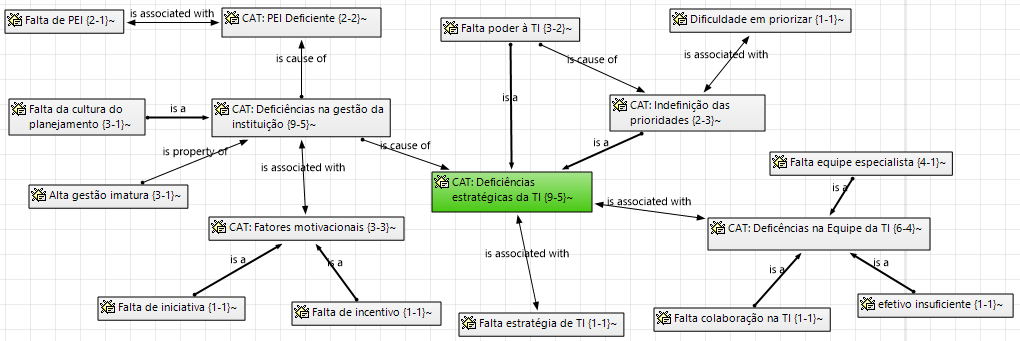
\includegraphics[width=15cm, frame]{figuras/sc_grupo1.PNG}
\caption{Esquema teórico do grupo 1 após a codificação seletiva.}
\label{figura:sc_grupo1}
\end{figure}

\begin{figure}[h!]
\centering % para centralizarmos a figura
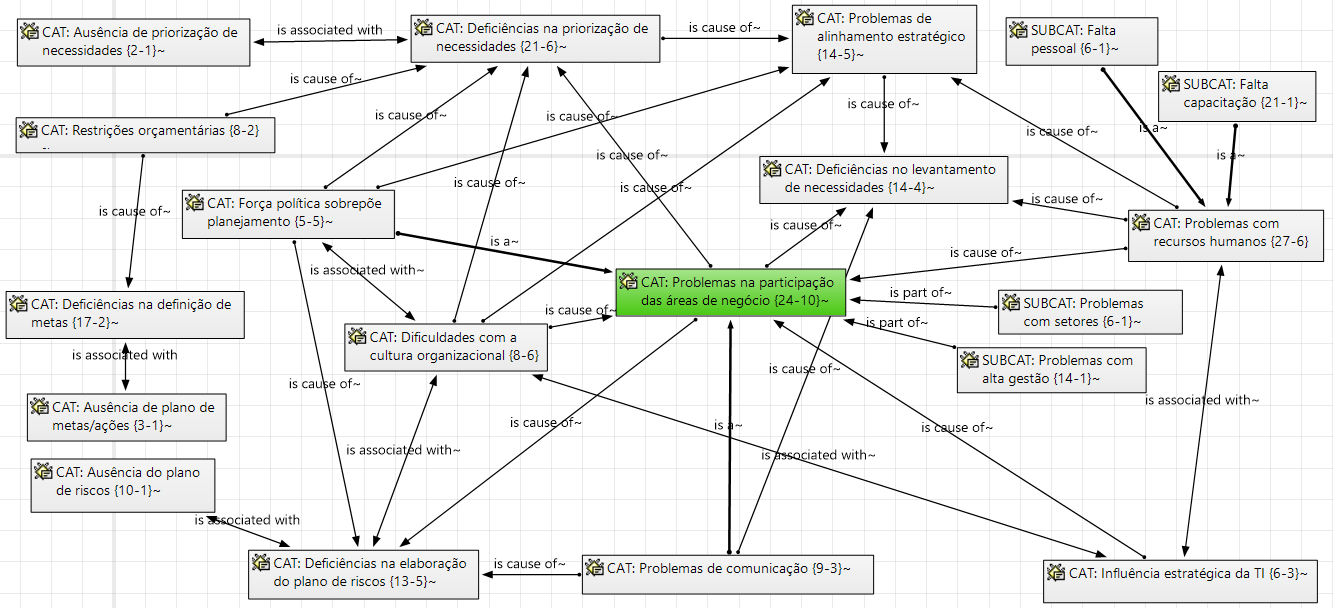
\includegraphics[width=15cm, frame]{figuras/sc_grupo2.PNG}
\caption{Esquema teórico do grupo 2 após a codificação seletiva.}
\label{figura:sc_grupo2}
\end{figure}



\section{Resultado: Teorias Fundamentadas nos Dados}
\label{secao:resultado_teorias}
Após a aplicação do método \textit{Grounded Theory}, foi possível visualizar as categorias centrais de cada grupo de dados e, através de seus relacionamentos e propriedades, traçar uma teoria para cada grupo pesquisado. Além dos esquemas teóricos, que representam graficamente a teoria central após as análises dos dados, uma teoria pode ser expressada através de um paradigma, contendo três elementos fundamentais: condição causal, fenômeno (categoria central) e consequência (questão da pesquisa) \cite{corbin:98}.

Uma teoria substantiva de qualidade deve estar isenta de arbitrariedade do pesquisador, sendo capaz de permitir seu livre escrutínio público por meio de auditorias que avaliem o pesquisador e o processo de pesquisa utilizado \cite{bandeira:03}.

Para o grupo 1, das instituições sem PDTI, a categoria central foi caracterizada como ``Deficiências estratégicas da TI''. Sua condição causal, ou seja, a razão que implica a categoria central foi caracterizada como ``nível baixo de maturidade em gestão''. A consequência disto é a ``ausência de planejamento de TI''. Diante disso, utilizando-se das propriedades das categorias envolvidas no paradigma causal, a teoria fundamentada nos dados sobre a ausência de um PDTI em uma instituição pode ser expressada da seguinte forma:

\textbf{Teoria para a ausência do PDTI nas instituições:} ``\textit{Uma instituição com baixo nível de maturidade em gestão não dá a devida importância à planos estratégicos e não reconhece a TI como parte estratégica da instituição. A área de TI, por sua vez, apresenta deficiências estratégicas como (a) baixo nível de influência da TI na instituição como um todo e (b) equipe inadequada em quantidade e em domínio de técnicas de planejamento; tais fatores impedem ou dificultam a elaboração do Plano Diretor de TI.}''

A Figura \ref{figura:paradigma1} apresenta um esquema teórico composto apenas dos códigos presentes na teoria para a ausência do PDTI nas instituições.

\begin{figure}[h!]
\centering % para centralizarmos a figura
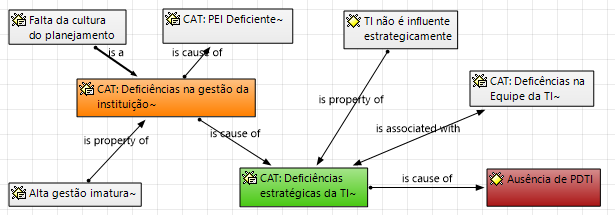
\includegraphics[width=13cm, frame]{figuras/paradigma1.PNG}
\caption{Esquema teórico da teoria 1.}
\label{figura:paradigma1}
\end{figure}


Para o grupo 2, das instituições com PDTI, a categoria central foi caracterizada como ``problemas na participação das áreas de negócio''. Sua condição causal, ou seja, a razão que implica a categoria central foi caracterizada como uma tríade de categorias: ``problemas de cultura organizacional'' + ``TI não reconhecida estrategicamente'' + ``problemas com recursos humanos''. A consequência disto são as ``dificuldades na elaboração do planejamento e PDTI com deficiências''. Diante disso, utilizando-se das propriedades das categorias envolvidas no paradigma causal, a teoria fundamentada nos dados sobre as dificuldades na elaboração de um PDTI em uma instituição pode ser expressada da seguinte forma:

\textbf{Teoria para as dificuldades na elaboração e deficiências do PDTI:} \textit{``Uma instituição que (i) possui membros que colocam interesses particulares e políticos acima dos interesses da instituição; (ii) não possui a percepção de que a TI é parte estratégica e (iii) não possuem recursos humanos devidamente capacitados para promover a cultura do planejamento, não apresenta o comprometimento e a participação satisfatória das áreas de negócio na composição do planejamento de TI. Tal participação das áreas de negócio é o fator que mais impacta nas dificuldades e deficiências apresentadas na elaboração do PDTI.''}

A Figura \ref{figura:paradigma2} apresenta um esquema teórico composto apenas dos códigos presentes na teoria para as dificuldades na elaboração e deficiências do PDTI.

\begin{figure}[h!]
\centering % para centralizarmos a figura
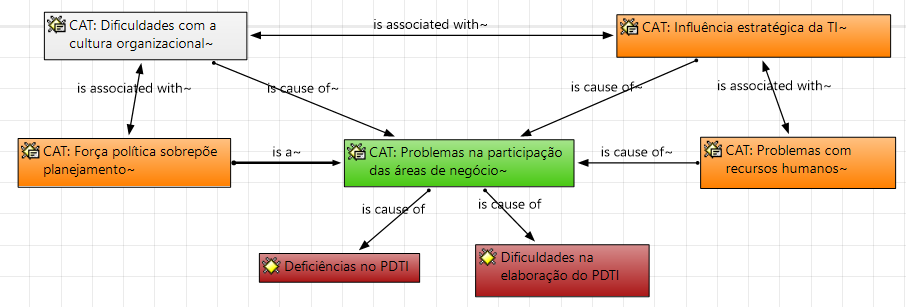
\includegraphics[width=13cm, frame]{figuras/paradigma2.PNG}
\caption{Esquema teórico da teoria 2.}
\label{figura:paradigma2}
\end{figure}

É possível verificar os passos da pesquisa que levaram às teorias apresentadas. O apêndice \ref{apendice:d_respostas_disserta} apresenta os dados na íntegra, conforme a respostas coletadas. O apêndice \ref{apendice:e_codigos} apresenta os códigos extraídos dos dados e os apêndices \ref{apendice:f_notas_ma} e \ref{apendice:h_notas_oc} apresentam as anotações feitas durante a fase de codificação aberta. Posteriormente, a fase de codificação axial, na qual descobre-se os relacionamentos entre os códigos, está descrita nas anotações presentes no apêndice \ref{apendice:i_notas_ac}.

\section{Avaliação dos Resultados}
\label{secao:avaliacao_resultados}
%Anexo B (contém as questões apenas)
O problema abordado neste trabalho exige que o pesquisador seja isento de hipóteses ou conclusões pré-concebidas, uma vez que a proposta desta pesquisa é permitir que os resultados sejam fielmente baseados nos dados coletados com os envolvidos no problema, garantindo que a conclusão seja o mais próxima possível da realidade. Na GT, a coleta dos dados, análise, formulação e a validação da teoria são reciprocamente relacionadas, em um processo indutivo de interpretação e em um processo de dedução e validação de proposições \cite{bandeira:03}.

Contudo, foi elaborado um questionário aplicado aos participantes da fase de coleta de dados. Tal questionário tem o objetivo de medir a aderência, através de escala de \textit{Likert}, da teoria resultante da pesquisa às dificuldades de planejamento de TI vivenciadas pelos respondentes.

Foram obtidas 32 avaliações de 23 instituições diferentes, de um total 37 instituições alvo. As avaliações foram divididas em dois grupos com perguntas específicas para cada grupo. O primeiro grupo é composto de membros de instituições que não possuem um PDTI, ao contrário do segundo grupo, composto por membros de instituições que já possuem um PDTI. O questionário aplicado nesta etapa da pesquisa é apresentado no \autoref{apendice:b_quest_avaliacao}.

Ao primeiro grupo foi apresentado a teoria sobre as razões que impedem a instituição de elaborar um PDTI. Em uma escala de zero a cinco, onde zero corresponde à ``discordo totalmente'' e cinco corresponde à ``concordo totalmente'', 100\% dos respondentes apontam que a teoria levantada é aderente à realidade. Deste total, 66,7\% concordam totalmente com a teoria. A Figura \ref{figura:grafico_ava_grupoSemPDTI} mostra a distribuição das respostas do primeiro grupo.


\begin{figure}[h]
\centering % para centralizarmos a figura
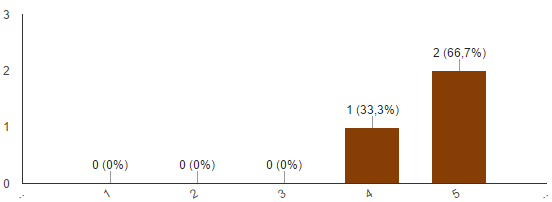
\includegraphics[width=10cm, frame]{figuras/grafico_ava_grupoSemPDTI.PNG}
\caption{Aderência à teoria sobre as razões da ausência de um PDTI}
\label{figura:grafico_ava_grupoSemPDTI}
\end{figure}

Ao segundo grupo foi apresentado a teoria sobre as dificuldades e deficiências encontradas em uma instituição ao elaborar seu PDTI. Em uma escala de zero a cinco, onde zero corresponde à ``discordo totalmente'' e cinco corresponde à ``concordo totalmente'', 79,3\% dos respondentes apontam que a teoria levantada é aderente à realidade. Enquanto 20,7\% optaram pela alternativa central da escala. A Figura \ref{figura:grafico_ava_grupoComPDTI} mostra a distribuição das respostas do segundo grupo.

\begin{figure}[h]
\centering % para centralizarmos a figura
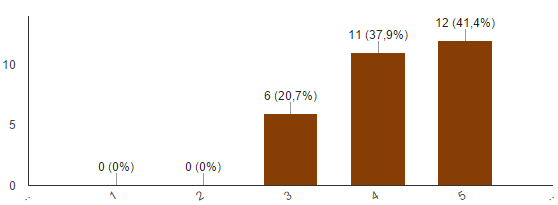
\includegraphics[width=10cm, frame]{figuras/grafico_ava_grupoComPDTI.PNG}
\caption{Aderência à teoria sobre as dificuldades na elaboração do PDTI}
\label{figura:grafico_ava_grupoComPDTI}
\end{figure}

Apesar de não ter atingido 100\% dos respondentes da coleta inicial de dados, os resultados apresentados no questionário de avaliação das teorias se mostraram, de forma geral, aderentes às teorias fundamentadas nos dados. Este resultado corrobora com os princípios da \textit{Grounded Theory}, que preza pelo empirismo no intuito de apresentar uma teoria próxima à realidade. Em outras palavras, os respondentes se viram representados na teoria.

\section{Considerações}
O processo de análise dos dados utilizando \textit{Grounded Theory} requer procedimentos metódicos e um profundo exercício de imparcialidade. Contudo, foi possível seguir os princípios da GT para atingir o objetivo da pesquisa.

Com o apoio da GT foi possível obter uma teoria fundamentada em dados que evidencia as principais causas das dificuldades de planejamento de TI nas instituições. Além disso, também através de uma teoria fundamentada nos dados, identificou-se as principais motivações que levam ao não cumprimento da determinação de se estabelecer o PDTI.

As teorias aqui apresentadas respondem à questão de pesquisa: ``apesar da obrigatoriedade e dos conhecidos benefícios, o planejamento de TI não é realizado satisfatoriamente nos órgãos públicos federais. A atividade de planejamento envolve aspectos técnicos e sociais, diante disso, pergunta-se: quais os fatores que dificultam o processo de elaboração do planejamento de TI e quais as relações entre tais fatores?''.

A descrição completa das teorias são as respostas da pergunta de pesquisa, contudo, de forma resumida pode-se responder a questão de pesquisa dividindo-a em duas partes:

1 - Quais os fatores que dificultam o processo de elaboração do planejamento de TI?\\
Resposta: Baseado na teoria fundamentada em dados, para as instituições que não conseguiram elaborar o PDTI, os fatores que dificultam este processo são (i) as deficiências na gestão da instituição, com baixo nível de maturidade em gestão estratégica; e principalmente (ii) as deficiências estratégicas da TI, ou seja, a área de TI não é reconhecida estrategicamente e possuem equipe inadequada em quantidade e competências para desenvolver atividades estratégicas.

Já nas instituições que possuem o PDTI, os fatores que dificultam o processo de elaboração passam por (i) influência política interna sobrepondo o planejamento; (ii) baixa influência estratégica da TI; (iii) problemas com recursos humanos em quantidade e capacidade para desenvolver as atividades de planejamento; e principalmente (iv) falta de comprometimento e participação satisfatória das áreas de negócio na elaboração do PDTI.

2 - Quais as relações entre os fatores?\\
Resposta: os fatores apresentam relação de causa e consequência, conforme esquematizado a seguir:
\\
\\
\textbf{Teoria 1:}\\
\textit{Condição causal:} Nível baixo de maturidade em gestão;\\
\textit{Fenômeno:} Deficiências estratégicas na TI;\\
\textit{Consequência:} Ausência de planejamento de TI.
\\
\\
\textbf{Teoria 2:}\\
\textit{Condição causal:} A tríade ``problemas de cultura organizacional'' + ``TI não reconhecida estrategicamente'' + ``problemas com recursos humanos'';\\
\textit{Fenômeno:} Problemas na participação das áreas de negócio;\\
\textit{Consequência:} Dificuldades na elaboração do planejamento e PDTI com deficiências.


Conclui-se que o método se mostrou eficaz em trazer à tona teorias que refletem os dados. Os resultados apresentados, teorias e avaliações, convergem para o cumprimento do objetivo desta pesquisa: elucidar o problema da elaboração do planejamento de TI nos órgãos federais identificando empiricamente os fatores e os relacionamentos que levam a este cenário. Diante disso, na seção seguinte são apresentadas sugestões de ações para minimizar os fatores que contribuem para as deficiências do planejamento de TI no setor público.